% !TeX program = lualatex
% ================================================================
% Polish Tier 3 Vocabulary Version of ConstructionsAndLoci
%
% Generated by the server using the following settings:
%
%   language            Polish (pol)
%   text direction      left to right
%   font                Noto Serif
%   fallback font       Noto Serif
%   built from          latex/worksheets/geometry/constructions/constructionsAndLoci.tex
%   vocabulary key      latex/worksheets/geometry/constructions/constructionsAndLoci/L2/pol/constructionsAndLoci_polishKey.tex
%   tier 3 vocabulary   green   RGB 0 128 0
%   English text        black   RGB 0 0 0
%   Polish text         purple  RGB 112 48 160
%   layout macros       version 3
%
% Please don't edit any information in this comment block - the server
% compares it against the current settings and rebuilds this file when
% they differ, so changes here would be overwritten. However, feel free
% to make updates to the LaTeX below if you want to edit it.
% ================================================================

\documentclass[12pt,a4paper]{article}
% ================================================================
% Copied from the English sheet this was translated from, so that
% anything it sets up for itself still works here
% ================================================================
\usepackage[a4paper,top=12mm,bottom=12mm,left=15mm,right=15mm]{geometry}
\usepackage[T1]{fontenc}
\usepackage{amsmath}
\usepackage{amssymb}
% A sans serif font with a single-storey a, as children write it. It is
% used for the mathematics as well as the text.
\usepackage{tgadventor}
\renewcommand*{\familydefault}{\sfdefault}
\usepackage[italic]{mathastext}
\usepackage{enumitem}
\usepackage{tikz}
\usepackage[most]{tcolorbox}

% ================================================================
% Constructions and loci.
%
% Pupils already know how to construct the perpendicular bisector of
% a line segment, the perpendicular to a line at a point on the line,
% and the perpendicular from a point to a line, so there are no
% worked examples.
%
% Pages 1 to 3 are assorted construction questions. Pages 1 and 2
% have each construction on its own, with the lines at different
% angles, and page 3 uses the constructions to find the height of a
% triangle, to draw a square and to find the centre of a circle.
%
% Pages 4 to 8 introduce loci. The first two loci questions mark some
% of the points that follow a rule before the locus is drawn, so that
% pupils see why the locus is a circle, and why the perpendicular
% bisector is the locus of the points equidistant from two points.
% The next question puts these two loci together to make a region.
% Then come the shortest distance from a point to a line (the
% perpendicular from the point), the points a fixed distance from a
% line (two parallel lines, drawn with perpendiculars at two points),
% and the points a fixed distance from a line segment. The scaffolding
% fades from there: a region with three rules and no steps, a mast
% the same distance from three villages, and a treasure map that ends
% with clues of the pupils' own.
%
% The sheet is eight sides of A4, so it can be printed as a booklet
% on two sheets of A3. The \newpage commands are placed so that no
% question is split across a page.
%
% Pupils construct on the sheet, so every diagram is drawn to scale
% (1 unit in TikZ is 1 cm). The sheet has to be printed at actual
% size: "fit to page" shrinks the diagrams and changes the answers
% that are measured. The answers are in a comment beside each
% question.
% ================================================================

\pagestyle{empty}
\setlength{\parindent}{0pt}
\setlength{\parskip}{0pt}
% Ragged right, so that the spaces between words are all the same, and
% no words broken across lines. A minipage sets the text justified
% again, so each side-by-side column starts with \raggedright as well.
\AtBeginDocument{\raggedright}
\hyphenpenalty=10000
\exhyphenpenalty=10000
\setlist[enumerate]{label=(\alph*), leftmargin=*, itemsep=7pt,
  topsep=4pt, parsep=0pt}
\setlist[itemize]{leftmargin=*, itemsep=3pt, topsep=4pt, parsep=0pt}

% The idea the loci questions are built on, boxed and only faintly
% tinted, so the sheet is cheap to print.
\newtcolorbox{keyidea}{colback=orange!3,colframe=orange!35,boxrule=0.6pt,
  left=6pt,right=6pt,top=5pt,bottom=5pt}

\newcommand{\sheettitle}[1]{\begin{center}{\LARGE\bfseries #1}\end{center}
  \vspace{-6pt}}
% An instruction for the questions after it.
\newcommand{\instruction}[1]{\par{\large\bfseries #1}\par\vspace{6pt}}

% The questions are numbered with a counter, so that they can be moved.
\newcounter{qn}
\newcommand{\q}{\refstepcounter{qn}\textbf{Q\theqn.}\ }

% An answer line at the right-hand end of a question, with the units
% after it: \answer{2cm}{cm}. It goes on the last line of the question
% if there is room, and on a line of its own if not. (This is the
% \signed macro from The TeXbook, with \hfill in place of \hfil so
% that it still reaches the right margin when the text is ragged
% right.)
\newcommand{\gapstrut}{\rule[-1.5mm]{0pt}{7.5mm}}
\newcommand{\answer}[2]{{\unskip\nobreak\hfill\penalty50
  \hskip2em\hbox{}\nobreak\hfill\gapstrut\underline{\hspace{#1}}\,#2%
  \parfillskip=0pt \finalhyphendemerits=0 \par}}
% A gap in a sentence.
\newcommand{\gap}[1]{\gapstrut\underline{\hspace{#1}}}
% A full-width line to write an explanation on.
\newcommand{\wline}{\par\vspace{16pt}\noindent\rule{\linewidth}{0.4pt}}

% ----------------------------------------------------------------
% Diagrams. Every one is drawn at actual size. The bounding box of
% each picture is set by hand, to leave room around the lines for the
% construction arcs.
\tikzset{
  given/.style={line width=0.7pt},
  extension/.style={line width=0.7pt, dash pattern=on 3pt off 2.5pt},
  lab/.style={inner sep=3pt},
  note/.style={font=\small, inner sep=2pt},
}
% A point labelled with a letter: \pt{(x,y)}{label position}{letter}.
\newcommand{\pt}[3]{\fill #1 circle (1.5pt); \node[lab,#2] at #1 {$#3$};}
% A point on a map, labelled with what it is and its letter:
% \place{(x,y)}{label position}{pond $P$}.
\newcommand{\place}[3]{\fill #1 circle (1.5pt); \node[lab,#2] at #1 {#3};}
% A diagram under a question, centred, without the space that the
% center environment puts round it.
\newenvironment{diagram}{\par\vspace{8pt}\centering}{\par}

% Characters this language's font has not got are borrowed from another,
% rather than being silently dropped - see docs/translated-sheet-latex.md
\directlua{%
  if luaotfload and luaotfload.add_fallback then
    luaotfload.add_fallback("eallatinfallback",
      { "Noto Serif:mode=harf;" })
  else
    tex.error("this luaotfload is too old to register a fallback font")
  end
}
\usepackage[english]{babel}
\babelprovide[import]{polish}
\babelfont[polish]{rm}[Renderer=Harfbuzz, BoldFont={Noto Serif}, ItalicFont={Noto Serif}, BoldItalicFont={Noto Serif}, RawFeature={fallback=eallatinfallback}]{Noto Serif}
\babelfont[polish]{sf}[Renderer=Harfbuzz, BoldFont={Noto Serif}, ItalicFont={Noto Serif}, BoldItalicFont={Noto Serif}, RawFeature={fallback=eallatinfallback}]{Noto Serif}
\newcommand{\ealtext}[1]{\foreignlanguage{polish}{#1}}
\newcommand{\ealtextblock}[1]{{\raggedright\foreignlanguage{polish}{#1}\par}}
% ================================================================
% EAL layout helpers
% ================================================================
\usepackage{xcolor}

\definecolor{ealkeycolour}{RGB}{0,128,0}
\definecolor{ealenglish}{RGB}{0,0,0}
\definecolor{ealtwocolour}{RGB}{112,48,160}

\newsavebox{\ealboxen}
\newsavebox{\ealboxtr}
\newlength{\ealglosswd}
\newlength{\ealglossraise}
\setlength{\ealglossraise}{1.15em}

% a tier 3 word, in English and in translation alike
\newcommand{\ealkey}[1]{\textcolor{ealkeycolour}{#1}}
\newcommand{\ealkeytr}[1]{\textcolor{ealkeycolour}{\ealtext{#1}}}

% One translated word above one English word. Built from kernel
% primitives, never a tabular, which would break wherever the sheet
% loads array, booktabs or tabularx. The box is as wide as the wider of
% the two, so a long translation pushes its neighbours aside instead of
% overlapping them, and it claims its full height so a table row or a
% TikZ node makes room for it.
\newcommand{\ealgloss}[2]{%
  \sbox{\ealboxen}{\ealkey{#1}}%
  \sbox{\ealboxtr}{\small\textcolor{ealtwocolour}{\ealtext{#2}}}%
  \setlength{\ealglosswd}{\wd\ealboxen}%
  \ifdim\wd\ealboxtr>\ealglosswd\setlength{\ealglosswd}{\wd\ealboxtr}\fi
  \leavevmode
  \makebox[\ealglosswd][c]{%
    \makebox[0pt][c]{\usebox{\ealboxen}}%
    \makebox[0pt][c]{\raisebox{\ealglossraise}{\usebox{\ealboxtr}}}%
  }%
}

% opens up line spacing around a block of glosses, so the raised
% translations sit clear of the line above
\newenvironment{ealglossed}{\par\linespread{2.1}\selectfont\ignorespaces}{\par}

% a whole translated sentence above its English counterpart. block level,
% so it does not belong inside a tabular cell
\newcommand{\ealpara}[2]{%
  \par\addvspace{0.5\baselineskip}%
  {\color{ealtwocolour}\ealtextblock{#1}}%
  \penalty200
  {\color{ealenglish}#2\par}%
  \addvspace{0.5\baselineskip}%
}

\begin{document}

\begin{ealglossed}
\sheettitle{\ealgloss{Constructions}{Konstrukcje} and \ealgloss{Loci}{miejsca geometryczne}}
\end{ealglossed}

\begin{ealglossed}
\instruction{Use a ruler and a pair of \ealgloss{compasses}{cyrkla}.\\
Do not rub out your \ealgloss{construction}{konstrukcji} \ealgloss{arcs}{łuki}.}
\end{ealglossed}

\begin{ealglossed}
\q \ealgloss{Construct}{Skonstruuj} the \ealgloss{perpendicular bisector}{symetralną odcinka} of the \ealgloss{line segment}{odcinka} $AB$.
\end{ealglossed}

\begin{diagram}
\begin{tikzpicture}
  \useasboundingbox (-1,-3.4) rectangle (9,3.4);
  \draw[given] (0,0) -- (8,0);
  \pt{(0,0)}{left}{A}
  \pt{(8,0)}{right}{B}
\end{tikzpicture}
\end{diagram}

\vfill

\begin{ealglossed}
\q \ealgloss{Construct}{Skonstruuj} the \ealgloss{perpendicular}{prostopadłą} from the point $P$ to the line.
Then measure the \ealgloss{distance}{odległość} from $P$ to the line. \answer{2cm}{cm}
\end{ealglossed}

\begin{diagram}
\begin{tikzpicture}
  \useasboundingbox (-0.3,-3.3) rectangle (13,3.5);
  \draw[given] (0,0) -- (13,0);
  \pt{(8,3)}{above}{P}
\end{tikzpicture}
\end{diagram}

\vfill

\begin{ealglossed}
\q \ealgloss{Construct}{Skonstruuj} the \ealgloss{perpendicular}{prostopadłą} to the line at the point $Q$.
\end{ealglossed}

\begin{diagram}
\begin{tikzpicture}
  \useasboundingbox (-0.3,-0.8) rectangle (13,4.4);
  \draw[given] (0,0) -- (13,0);
  \pt{(4.5,0)}{below}{Q}
\end{tikzpicture}
\end{diagram}

\vfill
\newpage

\begin{ealglossed}
\q \ealgloss{Construct}{Skonstruuj} the \ealgloss{perpendicular}{prostopadłą} from the point $R$ to the line.
Then measure the \ealgloss{distance}{odległość} from $R$ to the line. \answer{2cm}{cm}
\end{ealglossed}

\begin{diagram}
\begin{tikzpicture}
  \useasboundingbox (-0.3,-1.3) rectangle (12.2,5);
  \begin{scope}[rotate=20]
    \draw[given] (0,0) -- (12.5,0);
    \pt{(6.5,-3)}{below}{R}
  \end{scope}
\end{tikzpicture}
\end{diagram}

\vfill

\noindent
\begin{minipage}[t]{0.48\linewidth}\raggedright
\begin{ealglossed}
\q \ealgloss{Construct}{Skonstruuj} the \ealgloss{perpendicular bisector}{symetralną odcinka} of the \ealgloss{line segment}{odcinka} $CD$.
Mark the \ealgloss{midpoint}{środek} $M$ of $CD$, and measure the length of $CM$.
\answer{2cm}{cm}
\end{ealglossed}

\vspace{6pt}
\centering
\begin{tikzpicture}
  \useasboundingbox (-4,-3.3) rectangle (4,3.3);
  \begin{scope}[rotate=40]
    \draw[given] (-3.5,0) -- (3.5,0);
    \pt{(-3.5,0)}{below left}{C}
    \pt{(3.5,0)}{above right}{D}
  \end{scope}
\end{tikzpicture}
\end{minipage}\hfill
\begin{minipage}[t]{0.48\linewidth}\raggedright
\begin{ealglossed}
\q \ealgloss{Construct}{Skonstruuj} the \ealgloss{perpendicular}{prostopadłą} to the line at the point $S$.
\end{ealglossed}

\vspace{6pt}
\centering
\begin{tikzpicture}
  \useasboundingbox (-4,-3.3) rectangle (4,3.3);
  \draw[given] (-1.2,-3.3) -- (-1.2,3.3);
  \pt{(-1.2,-0.6)}{left}{S}
\end{tikzpicture}
\end{minipage}

\vfill

\q
\begin{minipage}[t]{0.92\linewidth}\raggedright
\begin{ealglossed}
\begin{enumerate}[topsep=0pt]
  \item \ealgloss{Construct}{Skonstruuj} the \ealgloss{perpendicular}{prostopadłą} from the point $G$ to the line.
  \item \ealgloss{Construct}{Skonstruuj} the \ealgloss{perpendicular}{prostopadłą} to the line at the point $H$.
  \item What do you notice about your two \ealgloss{perpendiculars}{prostopadłych}? \answer{5cm}{}
\end{enumerate}
\end{ealglossed}
\end{minipage}

\begin{diagram}
\begin{tikzpicture}
  \useasboundingbox (-0.3,-2.9) rectangle (13.5,3.6);
  \draw[given] (0,0) -- (13.5,0);
  \pt{(3,2.5)}{above}{G}
  \pt{(9.5,0)}{below}{H}
\end{tikzpicture}
\end{diagram}

\vfill
\newpage

\noindent
\begin{minipage}[t]{0.48\linewidth}\raggedright
\begin{ealglossed}
\q The diagram shows the \ealgloss{triangle}{trójkąt} $ABC$.
\begin{enumerate}
  \item \ealgloss{Construct}{Skonstruuj} the \ealgloss{perpendicular}{prostopadłą} from $C$ to the \ealgloss{line segment}{odcinka} $AB$.
  \item The \ealgloss{perpendicular}{prostopadła} from $C$ to $AB$ is the \ealgloss{height}{wysokością} of the \ealgloss{triangle}{trójkąta}.
    Measure the \ealgloss{height}{wysokość}. \answer{1.6cm}{cm}
  \item The \ealgloss{base}{podstawa} $AB$ is 7\,cm long. Work out the \ealgloss{area}{pole} of the
    \ealgloss{triangle}{trójkąta} $ABC$. \answer{1.6cm}{cm$^2$}
\end{enumerate}
\end{ealglossed}

\vspace{8pt}
\centering
\begin{tikzpicture}
  \useasboundingbox (-0.8,-3.2) rectangle (7.8,4.6);
  \draw[given, line join=round] (0,0) -- (7,0) -- (2,4) -- cycle;
  \pt{(0,0)}{below left}{A}
  \pt{(7,0)}{below right}{B}
  \pt{(2,4)}{above}{C}
\end{tikzpicture}
\end{minipage}\hfill
\begin{minipage}[t]{0.48\linewidth}\raggedright
\begin{ealglossed}
\q The points $E$ and $F$ are on the line, 4\,cm apart.
\begin{enumerate}
  \item \ealgloss{Construct}{Skonstruuj} the \ealgloss{perpendicular}{prostopadłą} to the line at $E$, and the
    \ealgloss{perpendicular}{prostopadłą} to the line at $F$.
  \item Use your \ealgloss{compasses}{cyrkla} to mark the point $G$ on the \ealgloss{perpendicular}{prostopadłej}
    at $F$, and the point $H$ on the \ealgloss{perpendicular}{prostopadłej} at $E$, so that
    $EFGH$ is a \ealgloss{square}{kwadratem}.
  \item Measure the \ealgloss{diagonal}{przekątną} $EG$. \answer{1.6cm}{cm}
\end{enumerate}
\end{ealglossed}

\vspace{8pt}
\centering
\begin{tikzpicture}
  \useasboundingbox (-2.2,-0.8) rectangle (6.2,5);
  \draw[given] (-2.2,0) -- (6.2,0);
  \pt{(0,0)}{below}{E}
  \pt{(4,0)}{below}{F}
\end{tikzpicture}
\end{minipage}

\vfill

\noindent
\begin{minipage}[t]{0.47\linewidth}\raggedright
\begin{ealglossed}
\q A \textbf{\ealgloss{chord}{cięciwa}} is a \ealgloss{line segment}{odcinkiem} that joins two points on a
\ealgloss{circle}{kole}. The \ealgloss{centre}{środek} of this \ealgloss{circle}{koła} has not been marked.
\begin{enumerate}
  \item \ealgloss{Construct}{Skonstruuj} the \ealgloss{perpendicular bisector}{symetralną odcinka} of the \ealgloss{chord}{cięciwy} $PQ$.
  \item \ealgloss{Construct}{Skonstruuj} the \ealgloss{perpendicular bisector}{symetralną odcinka} of the \ealgloss{chord}{cięciwy} $RS$.
  \item The \ealgloss{centre}{środek} of the \ealgloss{circle}{koła} is the point where your two
    \ealgloss{perpendicular bisectors}{symetralne odcinków} cross. Mark it, and label it $O$.
  \item Measure the \ealgloss{radius}{promień} of the \ealgloss{circle}{koła}. \answer{1.6cm}{cm}
  \item Set your \ealgloss{compasses}{cyrkiel} to this \ealgloss{radius}{promień}, and draw a \ealgloss{circle}{koło} with
    \ealgloss{centre}{środkiem} $O$. Your \ealgloss{circle}{koło} should lie on top of the \ealgloss{circle}{koła} that is
    drawn.
\end{enumerate}
\end{ealglossed}
\end{minipage}\hfill
\begin{minipage}[t]{0.5\linewidth}\raggedright
\centering
\begin{tikzpicture}[baseline=(current bounding box.north)]
  \useasboundingbox (-3.9,-5.3) rectangle (5,3.9);
  \draw[given] (0,0) circle (3.5);
  \draw[given] (355:3.5) -- (65:3.5);
  \draw[given] (255:3.5) -- (325:3.5);
  \pt{(355:3.5)}{right}{P}
  \pt{(65:3.5)}{above right}{Q}
  \pt{(255:3.5)}{below left}{R}
  \pt{(325:3.5)}{below right}{S}
\end{tikzpicture}
\end{minipage}

\vfill
\newpage

\begin{ealglossed}
\sheettitle{\ealgloss{Loci}{miejsca geometryczne}}
\end{ealglossed}

\begin{keyidea}
\begin{ealglossed}
A \textbf{\ealgloss{locus}{miejsce geometryczne}} is the \ealgloss{set}{zbiór} of all the points that follow a rule.
The plural of \ealgloss{locus}{miejsca geometrycznego} is \textbf{\ealgloss{loci}{miejsca geometryczne}}.

\vspace{4pt}
To find a \ealgloss{locus}{miejsce geometryczne}, we mark some of the points that follow the rule and
look at the shape they make. Then we draw the \ealgloss{locus}{miejsce geometryczne} accurately with a
ruler and a pair of \ealgloss{compasses}{cyrklem}.
\end{ealglossed}
\end{keyidea}

\vfill

\noindent
\begin{minipage}[t]{0.55\linewidth}\raggedright
\begin{ealglossed}
\q The rule for this \ealgloss{locus}{miejsca geometrycznego} is that the point is 3\,cm from $C$.
\begin{enumerate}
  \item Use your ruler to mark 8 points that are 3\,cm from $C$.
  \item What shape do your points make? \answer{2.8cm}{}
  \item Use your \ealgloss{compasses}{cyrkla} to draw the \ealgloss{locus}{miejsce geometryczne} of the points that are
    3\,cm from $C$.
  \item The points that are less than 3\,cm from $C$ fill the inside
    of your \ealgloss{circle}{koła}. A \ealgloss{set}{zbiór} of points that fills an \ealgloss{area}{pole} is called a
    \textbf{\ealgloss{region}{obszarem}}. Shade the \ealgloss{region}{obszar} of the points that are less than
    3\,cm from $C$.
\end{enumerate}
\end{ealglossed}
\end{minipage}\hfill
\begin{minipage}[t]{0.42\linewidth}\raggedright
\centering
\begin{tikzpicture}[baseline=(current bounding box.north)]
  \useasboundingbox (-3.6,-3.6) rectangle (3.6,3.6);
  \pt{(0,0)}{below}{C}
\end{tikzpicture}
\end{minipage}

\vfill

\noindent
\begin{minipage}[t]{0.55\linewidth}\raggedright
\begin{ealglossed}
\q A point is \textbf{\ealgloss{equidistant}{równoodległy}} from $A$ and $B$ when it is the
same \ealgloss{distance}{odległości} from $A$ as it is from $B$.
\begin{enumerate}
  \item Set your \ealgloss{compasses}{cyrkiel} to 4\,cm. Draw an \ealgloss{arc}{łuk} with \ealgloss{centre}{środkiem} $A$, and
    an \ealgloss{arc}{łuk} with \ealgloss{centre}{środkiem} $B$, so that the \ealgloss{arcs}{łuki} cross above $AB$ and below
    $AB$. Mark the two points where the \ealgloss{arcs}{łuki} cross. Each of these
    points is 4\,cm from $A$ and 4\,cm from $B$, so it is \ealgloss{equidistant}{równoodległy}
    from $A$ and $B$.
  \item Do the same with your \ealgloss{compasses}{cyrklem} set to 5\,cm.
  \item Mark the point on the \ealgloss{line segment}{odcinku} $AB$ that is \ealgloss{equidistant}{równoodległy}
    from $A$ and $B$.
  \item Use your ruler to draw a straight line through your points.
    This line is the \ealgloss{locus}{miejscem geometrycznym} of the points that are \ealgloss{equidistant}{równoodległe} from $A$
    and $B$. Which \ealgloss{construction}{konstrukcja} draws this line?
    \wline
  \item Shade the \ealgloss{region}{obszar} of the points that are closer to $A$ than
    to $B$.
\end{enumerate}
\end{ealglossed}
\end{minipage}\hfill
\begin{minipage}[t]{0.42\linewidth}\raggedright
\centering
\begin{tikzpicture}[baseline=(current bounding box.north)]
  \useasboundingbox (-0.75,-4.6) rectangle (6.75,4.6);
  \draw[given] (0,0) -- (6,0);
  \pt{(0,0)}{left}{A}
  \pt{(6,0)}{right}{B}
\end{tikzpicture}
\end{minipage}

\vfill
\newpage

\noindent
\begin{minipage}[t]{0.47\linewidth}\raggedright
\begin{ealglossed}
\q The map shows two lighthouses, $L$ and $M$. The \ealgloss{scale}{skala} of the map
is 1\,cm to 2\,km. A boat is less than 7\,km from the lighthouse $L$,
and it is closer to the lighthouse $M$ than to the lighthouse $L$.
\begin{enumerate}
  \item How many centimetres on the map is 7\,km? \answer{1.6cm}{cm}
  \item Draw the \ealgloss{locus}{miejsce geometryczne} of the points that are 7\,km from $L$.
  \item \ealgloss{Construct}{Skonstruuj} the \ealgloss{locus}{miejsce geometryczne} of the points that are \ealgloss{equidistant}{równoodległe} from
    $L$ and $M$.
  \item Shade the \ealgloss{region}{obszar} where the boat could be.
\end{enumerate}
\end{ealglossed}
\end{minipage}\hfill
\begin{minipage}[t]{0.5\linewidth}\raggedright
\centering
\begin{tikzpicture}[baseline=(current bounding box.north)]
  \useasboundingbox (-3.8,-3.8) rectangle (5.2,3.8);
  \pt{(0,0)}{below}{L}
  \pt{(4.5,1.2)}{below}{M}
\end{tikzpicture}
\end{minipage}

\vfill

\begin{ealglossed}
\q The map shows a farmhouse $F$ and a straight road. The \ealgloss{scale}{skala} of
the map is 1\,cm to 100\,m. The farmer wants to build a straight track
from the farmhouse to the road, and wants the track to be as short as
possible.
\begin{enumerate}
  \item Use your ruler to draw three different straight tracks from
    $F$ to the road. Measure each one.

    \vspace{2pt}
    Track 1: \gap{1.6cm}\,cm \qquad Track 2: \gap{1.6cm}\,cm
    \qquad Track 3: \gap{1.6cm}\,cm
  \item \ealgloss{Construct}{Skonstruuj} the \ealgloss{perpendicular}{prostopadłą} from $F$ to the road, and measure
    it. \answer{1.6cm}{cm}
  \item Fill in the gap: the shortest \ealgloss{distance}{odległość} from a point to a line
    is along the \gap{3.4cm} from the point to the line.
  \item How long is the shortest track in real life? \answer{1.6cm}{m}
\end{enumerate}
\end{ealglossed}

\begin{diagram}
\begin{tikzpicture}
  \useasboundingbox (-0.3,-3) rectangle (15.2,5.4);
  \begin{scope}[rotate=8]
    \draw[given] (0,0) -- (15,0);
    \node[note, below, rotate=8] at (13.4,0) {road};
    \begin{scope}[shift={(5.5,3.5)}]
      \draw[line width=0.5pt, line join=round, fill=white]
        (-1.2,0.15) rectangle (-0.45,0.65)
        (-1.3,0.65) -- (-0.825,1.05) -- (-0.35,0.65);
    \end{scope}
    \pt{(5.5,3.5)}{right}{F}
  \end{scope}
\end{tikzpicture}
\end{diagram}

\vfill
\newpage

\begin{ealglossed}
\q The \ealgloss{distance}{odległość} from a point to a line is the shortest \ealgloss{distance}{odległością}, so
it is measured along the \ealgloss{perpendicular}{prostopadłej}. In this question we draw the
\ealgloss{locus}{miejsce geometryczne} of the points that are 2\,cm from the line.
\begin{enumerate}
  \item \ealgloss{Construct}{Skonstruuj} the \ealgloss{perpendicular}{prostopadłą} to the line at the point $P$.
    Mark the two points on your \ealgloss{perpendicular}{prostopadłej} that are 2\,cm from $P$,
    one on each side of the line.
  \item Do the same at the point $Q$.
  \item Use your ruler to draw a straight line through the two points
    above the line, and another through the two points below the line.
    These two lines are the \ealgloss{locus}{miejscem geometrycznym} of the points that are 2\,cm from the
    line. They are \textbf{\ealgloss{parallel}{równoległe}} to the line: they stay the same
    \ealgloss{distance}{odległość} from it, and never meet it.
\end{enumerate}
\end{ealglossed}

\begin{diagram}
\begin{tikzpicture}
  \useasboundingbox (-0.3,-3.1) rectangle (14.3,3.1);
  \draw[given] (0,0) -- (14,0);
  \pt{(3.5,0)}{below right}{P}
  \pt{(10.5,0)}{below right}{Q}
\end{tikzpicture}
\end{diagram}

\vfill

\begin{ealglossed}
\q The diagram shows the \ealgloss{line segment}{odcinek} $XY$. The dashed lines carry on
the line through $X$ and $Y$. In this question we draw the \ealgloss{locus}{miejsce geometryczne} of
the points that are 2\,cm from the \ealgloss{line segment}{odcinka} $XY$.
\begin{enumerate}
  \item \ealgloss{Construct}{Skonstruuj} the \ealgloss{perpendicular}{prostopadłą} to the line at $X$, and the
    \ealgloss{perpendicular}{prostopadłą} to the line at $Y$.
  \item Mark the points on each \ealgloss{perpendicular}{prostopadłej} that are 2\,cm from $XY$.
    Join them to draw two \ealgloss{line segments}{odcinki} that are \ealgloss{parallel}{równoległe} to $XY$.
  \item For a point to the left of $X$, the closest point of the \ealgloss{line segment}{odcinka} $XY$ is $X$ itself. So the points on this side that are
    2\,cm from $XY$ are the points that are 2\,cm from $X$. Use your
    \ealgloss{compasses}{cyrkla} to draw them. Do the same to the right of $Y$.
  \item Priya says, ``The \ealgloss{locus}{miejsce geometryczne} of the points that are 2\,cm from $XY$
    is a \ealgloss{rectangle}{prostokątem}.'' Explain why Priya is wrong.
    \wline
    \wline
\end{enumerate}
\end{ealglossed}

\begin{diagram}
\begin{tikzpicture}
  \useasboundingbox (-3,-2.9) rectangle (9,2.9);
  \draw[extension] (-2.6,0) -- (0,0) (6,0) -- (8.6,0);
  \draw[given] (0,0) -- (6,0);
  \pt{(0,0)}{below left}{X}
  \pt{(6,0)}{below right}{Y}
\end{tikzpicture}
\end{diagram}

\vfill
\newpage

\noindent
\begin{minipage}[t]{0.37\linewidth}\raggedright
\begin{ealglossed}
\q The plan shows a garden. The \ealgloss{scale}{skala} of the plan is 1\,cm to 1\,m.
A beehive is going to be put in the garden, and it must follow all
three of these rules.
\begin{itemize}
  \item[--] The beehive must be more than 3\,m from the wall of the
    house.
  \item[--] Bees need water, so the beehive must be less than 4\,m
    from the pond $P$.
  \item[--] The beehive must be closer to the apple tree $T$ than to
    the bench $B$.
\end{itemize}
\vspace{4pt}
Shade the \ealgloss{region}{obszar} of the garden where the beehive can go.
\end{ealglossed}
\end{minipage}\hfill
\begin{minipage}[t]{0.6\linewidth}\raggedright
\raggedleft
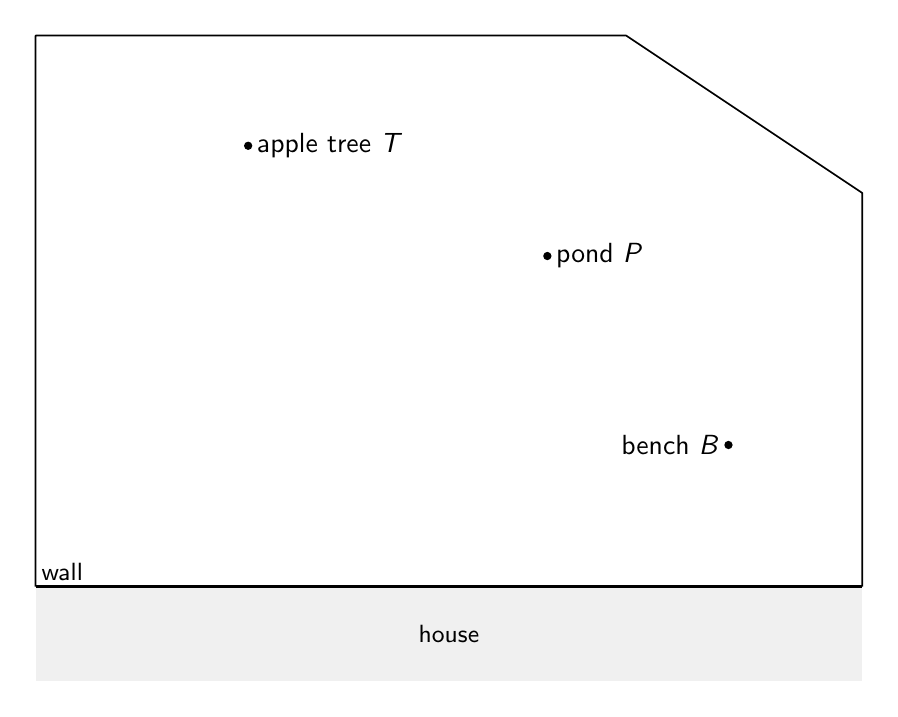
\begin{tikzpicture}[baseline=(current bounding box.north)]
  \useasboundingbox (-0.1,-1.3) rectangle (10.6,7.1);
  \fill[black!6] (0,-1.2) rectangle (10.5,0);
  \node[note] at (5.25,-0.6) {house};
  \draw[line width=0.6pt, line join=round]
    (0,0) -- (0,7) -- (7.5,7) -- (10.5,5) -- (10.5,0);
  \draw[line width=1.2pt] (0,0) -- (10.5,0);
  \node[note, above right] at (0,0) {wall};
  \place{(6.5,4.2)}{right}{pond $P$}
  \place{(2.7,5.6)}{right}{apple tree $T$}
  \place{(8.8,1.8)}{left}{bench $B$}
\end{tikzpicture}
\end{minipage}

\vfill

\noindent
\begin{minipage}[t]{0.47\linewidth}\raggedright
\begin{ealglossed}
\q Three villages, $A$, $B$ and $C$, are going to share a new phone
mast. The mast must be the same \ealgloss{distance}{odległości} from all three villages. The
\ealgloss{scale}{skala} of the map is 1\,cm to 2\,km.
\begin{enumerate}
  \item \ealgloss{Construct}{Skonstruuj} the \ealgloss{locus}{miejsce geometryczne} of the points that are \ealgloss{equidistant}{równoodległe} from
    $A$ and $B$.
  \item \ealgloss{Construct}{Skonstruuj} the \ealgloss{locus}{miejsce geometryczne} of the points that are \ealgloss{equidistant}{równoodległe} from
    $B$ and $C$.
  \item Mark the point $M$ where the mast must be built.
  \item \ealgloss{Construct}{Skonstruuj} the \ealgloss{locus}{miejsce geometryczne} of the points that are \ealgloss{equidistant}{równoodległe} from
    $A$ and $C$. What do you notice?
    \wline
  \item Explain why this happens.
    \wline
    \wline
  \item How far is the mast from each village in real life?
    \answer{1.6cm}{km}
\end{enumerate}
\end{ealglossed}
\end{minipage}\hfill
\begin{minipage}[t]{0.5\linewidth}\raggedright
\centering
\begin{tikzpicture}[baseline=(current bounding box.north)]
  \useasboundingbox (-4.5,-4.6) rectangle (4.5,5.4);
  \pt{(200:4)}{left}{A}
  \pt{(320:4)}{right}{B}
  \pt{(85:4)}{above}{C}
\end{tikzpicture}
\end{minipage}

\vfill
\newpage

\begin{ealglossed}
\q A treasure map has these two clues. The \ealgloss{scale}{skala} of the map is 1\,cm
to 10\,m.
\begin{itemize}
  \item[] \textbf{Clue 1:} The treasure is the same \ealgloss{distance}{odległości} from the
    oak tree $O$ as it is from the well $W$.
  \item[] \textbf{Clue 2:} The treasure is 40\,m from the standing
    stone $S$.
\end{itemize}
\end{ealglossed}

\begin{diagram}
\begin{tikzpicture}
  \useasboundingbox (-0.1,-0.1) rectangle (13.1,7.6);
  \draw[line width=0.6pt, rounded corners=4pt] (0,0) rectangle (13,7.5);
  \place{(2.5,1)}{right}{oak tree $O$}
  \place{(2,6)}{right}{well $W$}
  \place{(9,1)}{right}{standing stone $S$}
  \pt{(8.5,6.3)}{right}{X}
\end{tikzpicture}
\end{diagram}

\vspace{6pt}
\begin{ealglossed}
\begin{enumerate}
  \item Use both clues to mark the possible positions of the treasure.
  \item Write a third clue that tells you which of the positions is the
    treasure. Your clue must describe a \ealgloss{locus}{miejsce geometryczne}.
    \wline
    \wline
  \item More treasure is buried at the point $X$. Write some clues that
    lead to $X$ and to no other point on the map. Use as few clues as
    you can, and check your clues by \ealgloss{constructing}{konstruując} their \ealgloss{loci}{miejsca geometryczne} on the
    map.
    \wline
    \wline
    \wline
    \wline
\end{enumerate}
\end{ealglossed}

\vfill

\end{document}